% ============================================================
%  Semana 2 · Clase 2 — MasterClass (Nivelación)
%  Curso: Análisis y Visualización de Datos para la Toma de Decisiones
%
%  Formato de la sesión (3 h):
%    Hora 1 — Repaso relámpago + panorama del ecosistema de datos
%    Hora 2 — Fuentes, calidad de datos y formulación del problema
%    Hora 3 — Laboratorio: notebooks/lab-diagnostico-y-mapa-fuentes.ipynb
%
%  Compilar (dos veces) directamente desde esta carpeta:
%    xelatex semana02-clase02.tex
%    xelatex semana02-clase02.tex
% ============================================================
\documentclass[aspectratio=169,11pt]{beamer}

\usepackage{../../../plantilla/beamerthemeesumer}
\usetheme{esumer}

\usepackage[spanish]{babel}
\usepackage{booktabs}
\usepackage{graphicx}

% ---------------- DATOS DE LA CLASE ----------------
\title{MasterClass (Nivelación)}
\subtitle{Panorama del ecosistema de datos}
\author{Docente: Cristian A. Jimenez C., MSc}
\date{Sep 8 al 13}

\setmodulo{Módulo 1: Explorar (Fundamentos y Consulta de Datos)}
\setsemana{2}
\setclase{2}
\setfechaclase{Sep 8 al 13}
\setmodalidad{Presencial}
% -----------------------------------------------------

\graphicspath{{figuras/}}

\begin{document}

{
\setbeamertemplate{footline}{}
\begin{frame}[plain]
  \titlepage
\end{frame}
}

\begin{frame}{Agenda de hoy (3 horas)}
  \begin{columns}[T,onlytextwidth]
    \column{0.32\textwidth}
    \begin{block}{Hora 1}
      \small Repaso relámpago + panorama del ecosistema de datos
    \end{block}
    \column{0.32\textwidth}
    \begin{block}{Hora 2}
      \small Fuentes, calidad de datos y formulación del problema
    \end{block}
    \column{0.32\textwidth}
    \begin{block}{Hora 3}
      \small Laboratorio: diagnóstico + mapa de fuentes de tu proyecto
    \end{block}
  \end{columns}
  \vspace{0.5cm}
  \small Al final de hoy tendrás el \textbf{problema y la pregunta
  analítica inicial} de tu proyecto integrador.
\end{frame}

% ============================================================
\section{Hora 1 — Repaso y panorama}
% ============================================================
\begin{frame}{Recordemos la Clase 1}
  \begin{columns}[T,onlytextwidth]
    \column{0.48\textwidth}
    \textbf{La pirámide DIKW}
    \begin{itemize}
      \small
      \item Datos $\to$ Información $\to$ Conocimiento $\to$ Sabiduría.
      \item Sin contexto, un dato no vale mucho.
    \end{itemize}
    \column{0.48\textwidth}
    \textbf{El ciclo de vida del dato}
    \begin{itemize}
      \small
      \item Captura $\to$ Almacenamiento $\to$ Procesamiento $\to$ Análisis $\to$ Decisión.
      \item Hoy profundizamos en la \textbf{captura}: de dónde vienen los datos.
    \end{itemize}
  \end{columns}
\end{frame}

\begin{frame}{El ecosistema de datos de una empresa}
  \begin{columns}[T,onlytextwidth]
    \column{0.48\textwidth}
    \textbf{¿Quién participa?}
    \begin{itemize}
      \small
      \item Áreas que \textbf{generan} datos: ventas, operaciones, servicio al cliente.
      \item Áreas que \textbf{gestionan} datos: TI, sistemas.
      \item Áreas que \textbf{usan} datos: dirección, mercadeo, finanzas.
    \end{itemize}
    \column{0.48\textwidth}
    \textbf{¿Con qué herramientas?}
    \begin{itemize}
      \small
      \item Bases de datos y hojas de cálculo (dónde vive el dato).
      \item Python / SQL (cómo se explora y transforma).
      \item Power BI (cómo se comunica).
    \end{itemize}
  \end{columns}
  \vspace{0.25cm}
  \small Este curso te da una probada de cada rol: vas a capturar,
  limpiar, analizar y comunicar datos tú mismo.
\end{frame}

% ============================================================
\section{Hora 2 — Fuentes, calidad y problema}
% ============================================================
\begin{frame}{Fuentes internas y externas}
  \begin{center}
    
\includegraphics[width=0.92\textwidth]{figura_fuentes_datos.pdf}
  \end{center}
  \vspace{0.2cm}
  \small Todo proyecto de datos empieza por mapear \textbf{de dónde} van a
  salir los datos — eso es justo lo que harás en el laboratorio de hoy.
\end{frame}

\begin{frame}{Datos personales y calidad: profundicemos}
  \begin{columns}[T,onlytextwidth]
    \column{0.42\textwidth}
    \vspace{0.15cm}
    \small
    \begin{itemize}
      \small
      \item \textbf{Completitud:} ¿faltan valores?
      \item \textbf{Exactitud:} ¿el valor es correcto?
      \item \textbf{Consistencia:} ¿coincide entre fuentes?
      \item \textbf{Oportunidad:} ¿está actualizado?
      \item \textbf{Unicidad:} ¿hay duplicados?
    \end{itemize}
    \begin{alertblock}{\small Dato personal $\ne$ dato libre}
      \small En Colombia, la Ley 1581 de 2012 regula el tratamiento de
      datos personales (\emph{habeas data}). Úsalos solo con un propósito
      claro y proporcional.
    \end{alertblock}
    \column{0.53\textwidth}
    \centering
    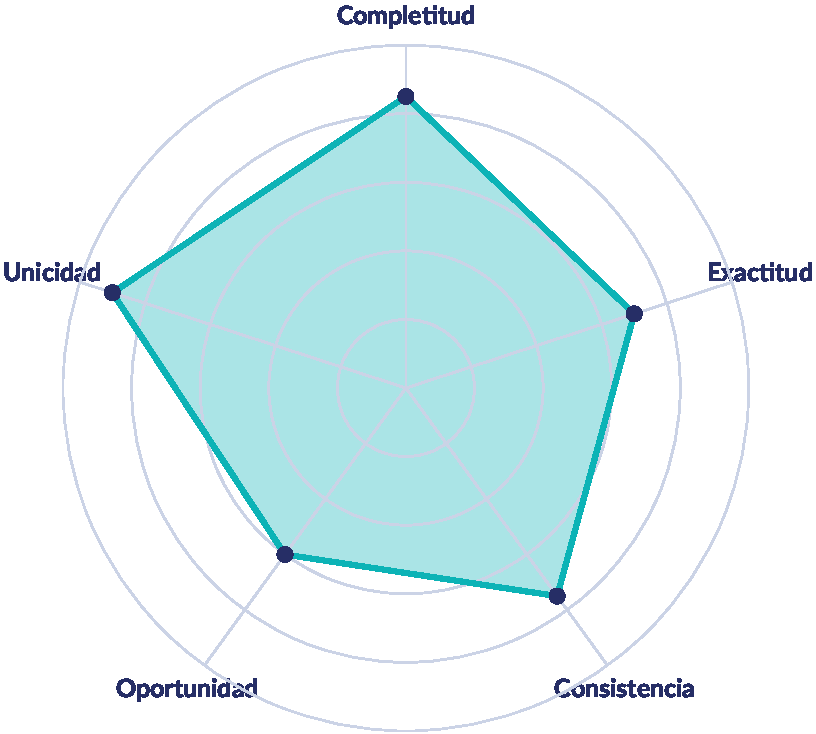
\includegraphics[width=0.95\textwidth]{figura_dimensiones_calidad.pdf}\\
    {\tiny \textcolor{gray}{Valores ilustrativos, no miden un dataset real.}}
  \end{columns}
\end{frame}

\begin{frame}{De un contexto a una métrica de éxito}
  \begin{center}
    
\includegraphics[width=\textwidth]{figura_formulacion_problema.pdf}
  \end{center}
  \vspace{0.25cm}
  \small Este es el mismo framework que usarás en el laboratorio para tu
  \textbf{proyecto integrador}.
\end{frame}

\begin{frame}{Ejemplo guiado}
  \begin{columns}[T,onlytextwidth]
    \column{0.19\textwidth}
    \small\textbf{Contexto}
    \column{0.19\textwidth}
    \small\textbf{Problema}
    \column{0.21\textwidth}
    \small\textbf{Pregunta analítica}
    \column{0.19\textwidth}
    \small\textbf{Datos necesarios}
    \column{0.19\textwidth}
    \small\textbf{Métrica de éxito}
  \end{columns}
  \vspace{0.15cm}
  \begin{columns}[T,onlytextwidth]
    \column{0.19\textwidth}
    \tiny Tienda de ropa con 5 sedes en Medellín.
    \column{0.19\textwidth}
    \tiny Las ventas bajaron 12\% el último trimestre.
    \column{0.21\textwidth}
    \tiny ¿En qué sedes y categorías cayó más la venta, y coincide con algún cambio de precio o inventario?
    \column{0.19\textwidth}
    \tiny Ventas por sede/categoría/mes, inventario, lista de precios.
    \column{0.19\textwidth}
    \tiny Identificar la(s) sede(s)/categoría(s) causantes de al menos el 60\% de la caída.
  \end{columns}
\end{frame}

% ============================================================
\section{Hora 3 — Laboratorio}
% ============================================================
\begin{frame}{Laboratorio: diagnóstico y mapa de fuentes}
  \begin{columns}[T,onlytextwidth]
    \column{0.55\textwidth}
    \textbf{Objetivo}
    \begin{itemize}
      \small
      \item Autodiagnóstico rápido de conceptos de la Clase 1.
      \item Mapear las fuentes de datos de tu proyecto integrador.
      \item Redactar tu \textbf{problema y pregunta analítica inicial}
        con el framework de hoy.
    \end{itemize}
    \column{0.4\textwidth}
    \begin{exampleblock}{Cuaderno}
      \small \texttt{notebooks/}\\ \texttt{lab-diagnostico-y-mapa-}\\\texttt{fuentes.ipynb}
    \end{exampleblock}
  \end{columns}
  \vspace{0.3cm}
  \small Trabajo individual sobre tu propio caso. El docente circula
  resolviendo dudas y retroalimentando las preguntas analíticas.
\end{frame}

\section{Cierre}
\begin{frame}{Cierre}
  \begin{itemize}
    \item Próxima sesión: \textbf{Fundamentos de estadística descriptiva} (Semana 2, virtual).
    \item Entregable de hoy: problema + pregunta analítica inicial (quedan como semilla del proyecto integrador).
    \item Dudas y comentarios.
  \end{itemize}
\end{frame}

{
\setbeamertemplate{footline}{}
\begin{frame}[plain]
  \begin{tikzpicture}[remember picture,overlay]
    \fill[esumerNavy] (current page.south west) rectangle (current page.north east);
    \node at (current page.center) {\color{white}\Huge\bfseries ¡Gracias!};
  \end{tikzpicture}
\end{frame}
}

\end{document}
